% disc.tex
\chapter{Analyse numérique}

\section{Opérateur de filtrage en dimension 1}

Lors de la discrétisation via un schéma aux différences finies et suite à la discrétisation en temps, des oscillations parasites du type "+1/-1" peuvent apparaître. Il s'agit de phénomènes haute fréquences qui peuvent provoquer des instabilités numériques. 

Si $\mathfrak{u}$ est une fonction de grille périodique, on note le filtre passe-bas $\mathcal{F}\mathfrak{u}$. Dans la pratique, nous cherchons $\mathcal{F}$ sous la forme 

\begin{equation}
\mathcal{F} = \gsum_{k=0}^F a_k \dfrac{\tau_k + \tau_{-k}}{2}
\label{eq:ftr}
\end{equation}

Les coefficients $(a_k)_{0 \leq k \leq F}$ sont déterminés de manière à supprimer les phénomènes oscillants hautes fréquences (figure \ref{fig:hf_waves}) de la formes $\mathfrak{u}$ avec 
\begin{equation}
\mathfrak{u}_j = (-1)^j
\end{equation}

\begin{figure}[htbp]
\begin{center}
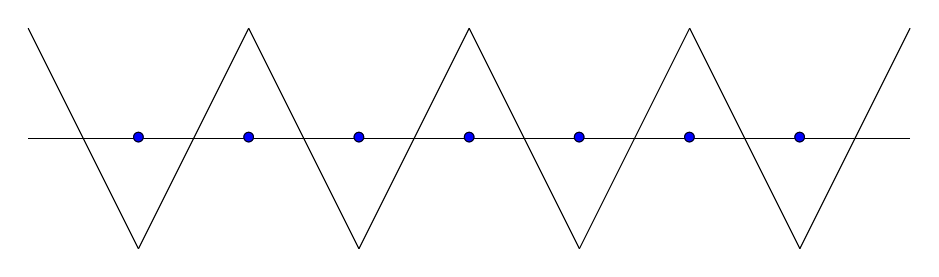
\begin{tikzpicture}[scale=1.4]
	\draw (-4,1) -- (-3,-1) ;
	\draw (-3,-1) -- (-2,1) ;
	\draw (-2,1) -- (-1,-1) ;
	\draw (-1,-1) -- (0,1) ;
	\draw (0,1) -- (1,-1) ;
	\draw (1,-1) -- (2,1) ;
	\draw (2,1) -- (3,-1) ;
	\draw (3,-1) -- (4,1) ;
	
	\draw (4,0) -- (-4,0) ;
	\foreach \k in {-3,...,3}
		{\draw  (\k,0) node[color=blue] {$\bullet$} ;
	   	\draw (\k,0) node {$\circ$} ;
	   	}
\end{tikzpicture}
\end{center}
\caption{Ondes de type "+1/-1".}
\label{fig:hf_waves}
\end{figure}


En considérant cette fonction de grille, on cherche $(a_k)_{0\leq k \leq F}$ tels que $\mathcal{F} \mathfrak{u} = \mathfrak{0}$, soit :
\begin{equation}
\mathcal{F}\mathfrak{u}_i = \gsum_{k=0}^F a_k \dfrac{\mathfrak{u}_{i+k} + \mathfrak{u}_{i-k}}{2} = \gsum_{k=0}^F a_k  \dfrac{(-1)^{i+k} + (-1)^{i-k}}{2} = 0.
\end{equation}
Cette équation est équivalente à 
\begin{equation}
\gsum_{k=0}^F a_k (-1)^k = 0
\label{eq:ftr_ftrcond}
\end{equation}
La relation \eqref{eq:ftr_ftrcond} nous donne une condition alors qu'il y a $F+1$ paramètres à déterminer. Il reste $F$ degrés de libertés dans l'opérateur de filtrage. Le choix qui est fait est de maximiser l'ordre du filtrage de manière à perturber un minimum la donnée initiale tout en supprimant les ondes parasites.

Le filtre doit conserver les très basses fréquences, lorsque $\mathfrak{u} = \mathfrak{1}$, on doit alors $\mathcal{F}\mathfrak{u} = \mathfrak{1}$.
C'est à dire que les coefficients $(a_k)_{0 \leq k \leq F}$ vérifient la relation de consistance
\begin{equation}
\gsum_{k=0}^F a_k = 1
\label{eq:ftr_conscond}
\end{equation}

Enfin, on remarque que si $u : x \in \Omega \mapsto u(x) \in \mathbb{R}$ et si $u^*$ est la fonction de grille associée à $u$, alors on a 
\begin{equation}
\begin{array}{rcl}
u(x_i + kh) & = & u(x_i) + p k u'(x_j) + \cdots + \dfrac{(kh)^l}{l!}u^{(l)}(x_i) + \cdots +\dfrac{(kh)^{2F}}{2F!} u^{(2F)}(\xi_k)\\
u(x_i - kh) & = & u(x_i) - p k u'(x_j) + \cdots + \dfrac{(-kh)^l}{l!}u^{(l)}(x_i) + \cdots +\dfrac{(-kh)^{2F}}{2F!} u^{(2F)}(\eta_k)
\end{array}
\end{equation}
avec $\xi_k \in [x_i, x_i+kh]$ et $\eta_k \in [x_i-kh, x_i]$. Alors par combinaison linéaire en considérant \eqref{eq:ftr_conscond} vérifiée, 
\begin{equation}
\mathcal{F}u^* - u^* = \gsum_{l=1}^{2F-1} \gsum_{k=0}^F \dfrac{a_k}{2} \underbrace{\dfrac{(kh)^l + (-kh)^l}{l!}}_{=0 \text{ pour } l \text{ impair.}}u^{(l)}(x_i) + \gsum_{k=0}^F \dfrac{a_k}{2}\dfrac{(kh)^{2F}}{2F!} \left( u^{(2F)}(\xi_k) + u^{(2F)}(\eta_k) \right)
\end{equation}
Ainsi, la condition de précision est 
\begin{equation}
\gsum_{k=0}^F a_k k^{2l} = 0 \text{ pour } 1 \leq l \leq F-1.
\label{eq:ftr_prescond}
\end{equation}

\begin{theoreme}
Soit $F \in \mathbb{N}^{\star}$. Il existe un unique $(a_k)_{0 \leq k \leq F}$ tel que $\mathcal{F}$ soit à la fois consistant en vérifiant \eqref{eq:ftr_conscond}, précis en vérifiant \eqref{eq:ftr_prescond} et soit un filtre passe bas en satisfesant \eqref{eq:ftr_ftrcond}. L'erreur de troncature du filtre est alors donnée par 
\begin{equation}
\mathcal{F}u^* - u^* = h^{2F} \gsum_{k=0}^F \dfrac{a_k}{2} \dfrac{k^{2F}}{2F!} \left( u^{(2F)}(\xi_k) + u^{(2F)}(\eta_k) \right).
\end{equation}
\end{theoreme}

\begin{proof}
La forme de l'erreur de troncature a déjà été vue, il reste à prouver l'unicité.

Après avoir retiré \eqref{eq:ftr_ftrcond} à \eqref{eq:ftr_conscond}, dire qu'il existe une unique $(a_j)_{0 \leq j \leq J}$ satisfesant les conditions est équivalent à dire que la matrice

\begin{equation}
A=\begin{pmatrix}
1 &  1  &  1  &  1  &  1  &  1  & \cdots\\  
0 &  2  &  0  &  2  &  0  & 2  & \cdots\\
0 &  1  & 2^2 & 3^2 & 4^2 & 5^2 & \cdots\\
0 &  1  & 2^4 & 3^4 & 4^4 & 5^4 & \cdots\\
0 &  1  & 2^6 & 3^6 & 4^6 & 5^6 & \cdots\\
&&& \vdots &  \vdots &
\end{pmatrix} \in \mathcal{M}_{J+1} \left( \mathbb{R} \right)
\end{equation}
est inversible car $a = [a_0, a_1, \cdots, a_J]^T$ est solution de 
\begin{equation}
A a = e_1
\end{equation}
avec $e = [1,1/2, 0,\cdots,0]^T$. En développant la seconde ligne de $A$, on a
\begin{equation}
\det ( A ) = \begin{vmatrix} 
2  &  0  &  2  &  0  & 2  & \cdots\\
1  & 2^2 & 3^2 & 4^2 & 5^2 & \cdots\\
1  & 2^4 & 3^4 & 4^4 & 5^4 & \cdots\\
1  & 2^6 & 3^6 & 4^6 & 5^6 & \cdots\\
& & \vdots &  \vdots &
\end{vmatrix} = 2 \sum_{k=1}^{\lfloor\frac{F-1}{2}\rfloor} \Delta_{2k+1}
\end{equation}
avec $\Delta_k$ donné par
\begin{equation}
\Delta_k = \begin{vmatrix} 
1 & 2^2 & \cdots & (k-1)^2 & (k+1)^2 & \cdots\\
1 & 2^4 & \cdots & (k-1)^4 & (k+1)^4 & \cdots\\
1 & 2^6 & \cdots & (k-1)^6 & (k+1)^6 & \cdots\\
&&& \vdots &  \vdots &
\end{vmatrix} = \dfrac{((F-1)!)^2}{k^2} \begin{vmatrix} 
1 & 1 & \cdots & 1 & 1 & \cdots\\
1 & (2^2)^1 & \cdots & ((k-1)^2)^1 & ((k+1)^2)^1 & \cdots\\
1 & (2^2)^2 & \cdots & ((k-1)^2)^2 & ((k+1)^2)^2 & \cdots\\
&&& \vdots &  \vdots &
\end{vmatrix}
\end{equation}
On reconnait alors un déterminant de Van-Der-Monde, donc $\Delta_k = \prod_{1 \leq i < j \leq F-1} \left( \alpha_j - \alpha_i \right)$, avec 
\begin{equation}
\alpha_j = \left\lbrace
\begin{array}{ll}
j^2 & \text{ avec } 1 \leq j \leq k-1\\
(j+1)^2 & \text{ avec } k \leq j \leq J-2\\
\end{array}
\right.
\end{equation}
Alors si $i<j$, on a $\alpha_i < \alpha_j$, donc $\Delta_k>0$ et même $\det A$ est une somme de déterminants tous strictements positifs donc $\det A > 0$. $A$ est inversible et le résultat est prouvé.
\end{proof}
Quelques filtres particuliers sont donnés dans la table \ref{tab:filter} en fonction de leur ordre de précision.

\begin{table}[htbp]
\begin{center}
\begin{tabular}{|c||cccccc|}
\hline
\textbf{Ordre de précision} & $a_0$ & $a_1$ & $a_2$ & $a_3$ & $a_4$ & $a_5$ \\
\hline \hline
$2$ & $1/2$ & $1/2$ & & & & \\
\hline
$4$ & $10/16$ & $8/16$ & $-2/16$ & & & \\
\hline
$6$ & $44/64$ & $30/64$ & $-12/64$ & $2/64$ & & \\
\hline
$8$ & $186/256$ & $112/256$ & $-56/256$ & $16/256$ & $-2/256$ & \\
\hline
$10$ & $772/1024$ & $420/1024$ & $-240/1024$ & $90/1024$ & $-20/1024$ & $2/1024$ \\
\hline
\end{tabular}
\end{center}
\caption{Exemples de filtres de la forme \eqref{eq:ftr} et leur ordre de précision.}
\label{tab:filter}
\end{table}

Dans la suite, nous supposerons que $(a_k)_{0 \leq k \leq F}$ satisfait les conditions \eqref{eq:ftr_conscond}, \eqref{eq:ftr_prescond} et \eqref{eq:ftr_ftrcond}.
Les valeurs propres et fonctions propres de $\mathcal{F}$ sont issues de la proposition \ref{prop:eigen_P(tau)}. Le résultat est immédiat.

\begin{theoreme}
Les valeurs propres de $\mathcal{F}$ sont données par $\beta^k$ avec 
\begin{equation}
\beta^k = \gsum_{f=0}^F a_k \cos \left( \dfrac{2 \pi k f}{N} \right)
\end{equation}
pour tout $0 \leq k \leq N-1$, $\beta^k$ est associé à la fonction propre $\mathfrak{u}^k$ telle que 
\begin{equation}
\mathfrak{u}^k_j = \exp \left[ i j \dfrac{2 \pi k}{N} \right].
\end{equation}
\end{theoreme}

On définit le \textit{symbole} du filtre $\mathcal{F}$ par la fonction $\beta : \theta \in [0, \pi] \mapsto \beta(\theta) \in \mathbb{R}$ donnée par :
\begin{equation}
\beta( \theta ) = \gsum_{f=0}^F a_k \cos \left( f \theta \right)
\end{equation}

\begin{proposition}
Il existe un unique polynôme $P$ de degré $F$ tel que 
\begin{equation}
\beta(\theta) = P(\cos \theta )
\end{equation}
De plus,
\begin{equation}
P(x) = 1 -\dfrac{1}{(-2)^F} (X - 1)^F.
\end{equation}
\end{proposition}

\begin{proof}
Soit $\theta \in [0, \pi]$, 
\begin{equation}
\beta(\theta) = \gsum_{f=0}^F a_f \cos \left( f \theta \right) = \gsum_{f=0}^F a_f T_f ( \cos \theta )
\end{equation}
où $T_f \in \mathbb{R}_f [X]$ est le $k-$ieme polynome de Tchebytchev. 
Ainsi il existe $P \in \mathbb{R}_F [x]$ tel que $\beta( \theta ) = P( \cos \theta )$. Ce polynôme est unique. Montrons que 
\begin{equation}
P(x) = 1 -\dfrac{1}{(-2)^F} (X - 1)^F.
\end{equation}
convient.

\begin{itemize}
\item on montre facilement que 
\begin{equation}
P( \cos 0 ) = 1 -\dfrac{1}{(-2)^F} (\cos 0 - 1)^F = 1,
\end{equation}
de même,
\begin{equation}
P( \cos \pi ) = 1 -\dfrac{1}{(-2)^F} (\cos \pi - 1)^F 1 -\dfrac{(-2)^F}{(-2)^F} = 0.
\end{equation}
\item On rappelle la formule de Fàa Di Bruno permettant de calculer la dérivée $n-$ième d'une composée. Si $f$ et $g$ sont des fonctions régulières, on a 
\begin{equation}
\dfrac{d^n}{dx^n} \left( f \circ g \right)(x) = \gsum_{k=1}^n f^{(k)}\left( g(x) \right) B_{n,k}\left( g'(x), g''(x), \cdots , g^{n-k+1}(x) \right)
\end{equation}
où $B_{n,k}$ est un polynôme de Bell. En utilisant cette formule avec $f = P$ et $g = \cos$, évaluée en $\theta = 0$, on montre que :
\begin{equation}
\dfrac{d^n}{d\theta^n} \left( P \circ \cos \right)(0) = \gsum_{k=1}^n P^{(k)}\left(1\right) B_{n,k}\left( -1,0,1,0, \cdots\right)
\end{equation}
Or, $P^{(k)}\left(1\right) = 0$ pour tout $k \geq 1$. Donc 
\begin{equation}
\dfrac{d^n}{d\theta^n} \left( P \circ \cos \right)(0) = 0
\end{equation}
\end{itemize}
Le polynôme $P$ convient et 
\begin{equation}
\beta( \theta ) = 1 - \dfrac{1}{(-2)^F}(\cos \theta -1)^F.
\end{equation}
\end{proof}

\begin{proposition}
Pour tout $\theta \in [0, \pi]$, on a 
\begin{equation}
0 \leq \beta ( \theta ) \leq 1
\end{equation}
\end{proposition}

\begin{proof}
Supposons qu'il existe $\theta \in [0, \pi]$ tel que $\beta(\theta) < 0$ ou $\beta(\theta) > 1$. Comme $\beta(0)=1$ et $\beta(\pi) = 0$, il existe $\tilde{\theta} \in ]0, \pi[$ tel que 
\begin{equation}
\beta'(\tilde{\theta}) = - \sin \tilde{\theta} P'(\cos \tilde{\theta} ) = 0
\end{equation}
Or $\sin \tilde{\theta} \neq 0$ pour $\tilde{\theta} \in ]0, \pi[$.
De plus, 
\begin{equation}
P'(X) = \dfrac{F}{(-2)^F}(X-1)^{F-1}
\end{equation}
donc en prenant $X = \cos \tilde{\theta}$,
\begin{equation*}
P'(X) = 0 \Leftrightarrow \cos \tilde{\theta} = 1
\end{equation*}
Ce qui est impossible pour $\tilde{\theta} \in ]0, \pi[$. Donc par l'absurde, le résultat est vérifié.
\end{proof}












\section{Discrétisation temporelle}

\subsection{Discrétisation de Runge-Kutta d'ordre 4}

\subsection{Stabilité}

\subsection{Schéma filtré}















\section{Equation d'advection 1D}

\subsection{Discrétisation}

\subsection{Consistance et Stabilité}

\subsection{Relations de conservations}